% !TEX TS-program = pdflatex
% !TEX root = ../ArsClassica.tex

%************************************************
\chapter{Mathematical Model}
\label{chp:2-Model}
%************************************************

\section{Wind Farm Cable Problem Introduction}We have studied the Wind Farms Cable Problem, which is represented by a number of wind farms in the sea that produces energy; the power production needs to be routed by some cables to the substation and then directed to the coast.
To do that, each turbine must be connected through a cable to another turbine, and eventually to a substation.

This problem complexity if the cable routing problem is strongly NP-hard according to \cite{wfcp}. They have proved that the problem is NP-hard in two formulation. First, in the case where all turbines have the same power production and the nodes are not associated with points in the plane. Second, in the case where the turbines can have different power production and are associated with point in the plane. 

When designing a feasible cable routing it's necessarly to take in account a number of constraints. Here we list some of them and then we'll describe the mathematical model that realizes those constraints. Our model is based on the following requirements:

\begin{itemize}
\item since the energy flow is unsplittable, the energy flow leaving a turbine must be supported by a single cable; 
\item power losses should be avoided beacuse it will cause revenue losses in the future;
\item different cables, with different capacities and costs, are available; this means that it is important to choose the right cable to minimize the costs without affecting the revenues 
\item the energy flow on each connection cannot exceed the capacity of the installed cable;
\item due to the substation physical layout, a given maximum number of cables, say $C$, can be connected to each substation; 
\item cable crossing should be avoided. (we will discuss this problem in the next subsection)
\end{itemize}
Let $K$ denote the number of different types of cables that can be used and let $n$ be the number turbines. 

Definition of $y_{ij}$ :
\[
	y_{ij} =
   \begin{cases}
   1 \quad \mbox{if arc } (i,j) \mbox{ is constructed} \\
   0 \quad \mbox{otherwise.} 
   \end{cases}
   \forall \,i,j = 1, ..., n 
\]
\[
	y_{ii} = 0, \quad \forall i= 1, ... n 
\]
Definition of $x^k_{ij}$ :
\[
	x^k_{ij} =
   \begin{cases}
   1 \quad \mbox{if arc } (i,j) \mbox{ is constructed with cable type k} \\
   0 \quad \mbox{otherwise.} 
   \end{cases}
   \forall \,i,j = 1, ..., n \ \forall \ k = 1,... K
\]
Definition of $f_{ij}$ :
\[
	f_{ij} \geq 0, \quad \forall i,j= 1, ... n
\]

%\[
%y_{i,j} = \sum_{t \in T} x^t_{ij}, \quad (i,j) \in A
%\]
Objective function: 
\begin{equation}\label{eq:obj}
	\min{\sum^n_{i=1} \sum^n_{j=1} \sum^K_{k} cost(k) \cdot dist(i,j) \cdot x^k_{ij}}
\end{equation}

Constraints: 
\begin{equation}\label{eq:numberCable}
	\sum^n_{j = 1} y_{hj} = 
	\begin{cases}
   1 \quad \mbox{if } P_h \geq 0, \quad \forall h=1,...,n \\
   0 \quad \mbox{if } P_h = -1
   \end{cases}
\end{equation}

\begin{equation}\label{eq:basestation}
	\sum^n_{i =1} y_{ih} \leq C, \quad \forall h \ | \ P_h = -1
\end{equation}

\begin{equation}\label{eq:flux}
	\sum^n_{j=1} f_{hj} = \sum^n_{i=1} f_{ih}+ P_h, \quad \forall h \ | \ P_h \geq 0
\end{equation}

\begin{equation}\label{eq:oneCable}
	y_{ij} = \sum^K_{k=1} x^k_{ij}, \quad i,j = 1,...,n
\end{equation}

\begin{equation}\label{eq:capacity}
	\sum^K_{k=1} cap(k)x^k_{ij} \geq f_{ij}, \quad \forall i,j = 1,...,n
\end{equation}

[magari cambiare ordine qui sotto]\\
The objective function \ref{eq:obj} minimizes the total cable layout cost, where $dist(i, j)$ is the Euclidean distance between nodes $i$ and $j$ and $cost(k)$ is the unit cost for the cable $k$. 
Constraints \ref{eq:oneCable} impose that only one type of cable can be selected for each build arc.
Constraints \ref{eq:flux} are flow conservation constraints: the energy exiting each node $h$ is equal to the energy entering $h$ plus the power production of the node. 
Constraints \ref{eq:capacity} ensure that the flow does not exceed the capacity of the installed cable.
Constraints \ref{eq:numberCable} impose that only one cable can exit a turbine and that no one cable can exit from the substation. 
Constraint \ref{eq:basestation} imposes the maximum number of cables ($C$) that can enter in a substation, depending on the data of the instance. The image \ref{img:wfcp} shows an example of a graphical solution to the cable routing problem.

\begin{center}
	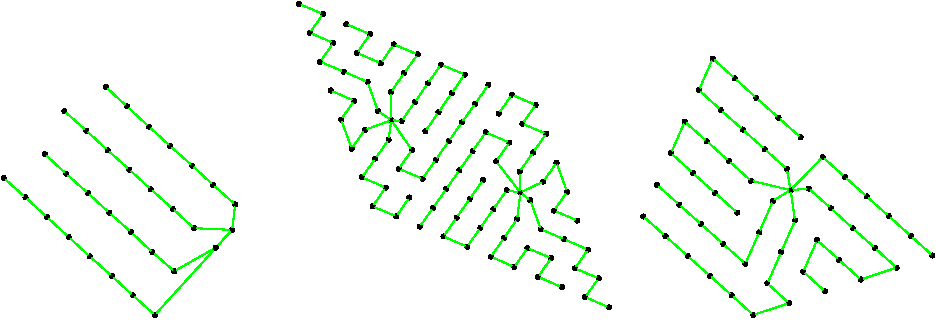
\includegraphics[scale=0.4]{Graphics/wfcp.png}
	\captionof{figure}{Example solutions to a cable routing problem}
	\label{img:wfcp}
\end{center}
	
\section{Crossing Cables}
According to \cite{wfcp}, an important constraint is that cable crossings should be avoided. In principle, cable crossing is not impossible, but is strongly discouraged in practice as building one cable on top of another is more expensive and increase the risks of cable damages.\\

In order to evaluate if two arches cross we used the Cramer Method: given the arc $a$ between $P_1$ and $P_2$ and the arc $b$ between $P_3$ and $P_4$. We define the coordinates of a general point as: $P_j = (X_i, y_i)$. \\
Using the Cramer method we have:
\[
{x \choose y} = {x_1 \choose y_1}+ \lambda {x_2 - x_1 \choose y_2 - y_1} \quad \lambda \in \ ]0, 1[
\]   
\[
{x \choose y} = {x_3 \choose y_3}+ \mu {x_4 - x_3 \choose y_4 - y_3} \quad \mu \in \ ]0, 1[
\]    
Then we evaluate if the determinant is equal to zero value; to do this in a calculator environment avoiding mistakes we will check if the determinant is smaller than a constant epsilon with value $\simeq 10^{-9}$. We can have two situations:
\begin{enumerate}
\item if $det=0 \quad \Rightarrow$ no crossing 
\item if $det \neq 0 \quad \Rightarrow (\lambda, \mu) \ if \ (\lambda \in \ ]0, 1[) \ \&\& \ (\mu \in \ ]0, 1[) \Rightarrow $ crossing
\end{enumerate}                                                   

[spiegareeee]!!!

\[
y(a,b)+ y(c,d) \leq 1, \quad \forall (a,b,c,d): [P_a, P_b] \ cross \ [P_c, P_d]
\]

